\documentclass{deliverablereport}
\usepackage{pdfpages}
\usepackage{pgfplots}
\pgfplotsset{compat=1.5}

\deliverable{hpc}{pari-hpc2}
\deliverydate{2019-08-31}
\duedate{2019-08-31 (M48)}

\author{Bill Allombert, Karim Belabas}

\begin{document}
\maketitle
\githubissuedescription
\tableofcontents

\section{Introduction and rationale}

The \Pari library is a state-of-the-art library for number theory,
developed at Bordeaux University. It is an important component of the \Sage
computational system: \Sage uses it for example to implement number fields
and elliptic curves. \Pari itself is a C library but it comes with a
command-line interface called \texttt{gp} which can be programmed in the GP
scripting language, and a GP-to-C compiler called GP2C. Together, these form
the software package \PariGP. This deliverable is about allowing,
simplifying, or spreading the use of parallel computation in the system.

In experimental number theory, many large computations are ``embarassingly
parallel'': no communication is needed between parallel tasks and there is
little data to pass from the main thread to the computing nodes. They usually
fit one of the following scenarios:
\begin{enumerate}
  \item exhaustive enumeration for theorem proving: for instance, asymptotic
    methods prove that all integers larger than some moderate bound $X$
    satisfy the theorem and we must check the remaining finitely many
    integers $n \leq X$. This generalizes to more complicated parameter sets
    as long as some theoretical proof leaves us with a finite
    moderately-sized space to enumerate.

  \item building databases: number theorists love building tables and
    databases of interesting objects, usually all (finitely many) objects
    of given ``kind'' and bounded ``size''. The motivation is for instance
    to infer general models from finite statistics or to test algorithms on
    large unbiased data sets. The $L$-functions and Modular Forms Database
    (LMFDB) is a prominent example.

  \item sampling: exploring a huge space until a favourable outcome occurs,
    e.g., a collision (as in the rho or ECM integer factoring method), or
    until sufficiently many data has been acquired to solve a problem by
    linear algebra (as in \emph{sieve} methods to factor integers or
    \emph{index calculus} algorithms to solve discrete logarithm problems).

  \item modular algorithms: where bounded integers are recognized by their
    congruence classes modulo sufficiently many primes and the Chinese
    Remainder Theorem (CRT), or interpolation algorithms where polynomials of
    bounded degrees are determined by sufficiently many values. The modular
    computations are independent of each other and offer a general speedup
    compared to a direct computation because they operate on much smaller
    inputs and do not suffer from coefficient explosion.
\end{enumerate}

In all these cases, most of the computational effort is easily split into
independent parts of roughly equal sizes. In cases 3) and 4),
post-processing the independent results may be non-trivial: integer
factorization and discrete logarithms end with a linear algebra problem in
huge dimensions; sophisticated quasi-linear time CRT or interpolation methods
are required for efficient modular reconstruction.

Now, typical number theorists have scant access to HPC clusters and use
personal machines. But even cheap laptops have 2 or 4 computing cores
nowadays. How can we ensure that \PariGP users get this expected two- or fourfold
improvement ? And make that $N$-fold if an $N$-cores cluster becomes
available ? Of course, we also need to limit the implementation effort:
maintaining three or more variants of each algorithm (single core machine,
multicore single machine, cluster) is not manageable.

This deliverable, a merger of subtask D5.10 and demonstrator D5.16 in the
submitted proposal, implements a generic parallel engine in the
\PariGP system, uses it inside the system (expecting speed gains) and
exports it for library users. The released \PariGP suite (PARI-2.12 at
\url{http://pari.math.u-bordeaux.fr/download.html}) makes those
improvements and new features available for the community, in particular
\Sage users and all software using the \Pari library.

More precisely, the MultiThread engine, or MT engine for short, transparently
supports: 1) sequential computation, 2) POSIX threads (for a single multicore
machine) and 3) Message Passing Interface (MPI, for clusters). It can be used
in two different ways:

\begin{itemize}
\item Explicit parallelism: the MT engine provides interfaces to launch
  subtasks in parallel and efficiently share global data with the tasks. The
  user must subdivide the tasks herself, handle load balancing and failures
  and recombine results, but she has complete control.

\item Implicit parallelism: a relevant selection of high-level system
  routines decide on their own to use explicit parallelism, or not. This is
  easier on the user but more complicated to handle, because there are many
  possible strategies and no automated algorithm can be optimal in all
  cases without some amount of user input: for instance, if routine $A$
  calls routine $B$ independently many times, it is easier and more efficient
  to parallelize $A$ and leave $B$ alone than to parallelize $B$. But how can
  the engine know that $A$ is going to invoke $B$ many times ? Or that the
  calls to $B$ have roughly the same cost (or not, in which case load
  balancing becomes non-trivial)?
\end{itemize}

\section{Work accomplished}
\subsection{Initial state at the start of the project}
Since PARI-2.7 (released 03/2014), it was already possible to build a
thread-safe PARI library and to use the standard POSIX threads interface in
separate autonomous C programs. The GP language also contained a handful of
parallel control structures, mirroring sequential equivalents, which
allowed the explicit scenario in the previous section: for instance, the
sequential \texttt{for} loop has a parallel \texttt{parfor} equivalent.

Two main difficulties with parallel computing in GP prevent an automatic
switch to the implicit paradigm: first, using the parallel machinery
involves overhead and it is hard to decide automatically whether
an arbitrary \texttt{for} loop will benefit or suffer; and second,
global variables (more generally, side effects) cause the usual difficulties.

\subsection{The generic MT engine}
The MT engine was written and finalized in 2015 and 2016 and is in
production since PARI-2.9 (released 11/2016). It supports sequential
evaluation (no parallelism), POSIX threads and MPI within the same code
base. The full suite is supported: GP2C correctly compiles GP code which is
making use of the GP parallel interface.

Since then, the engine has been extensively tested on Unix/Linux
desktop computers (up to 96 cores) and clusters (up to 128 nodes), and on
laptops running Linux, OSX and Windows 10 (Bash on Windows). As expected, in
embarassingly parallel algorithms, the measured speedup was essentially
linear in the number of available cores; in more complicated programs where
post-processing is not negligible, the gain is smaller.

User documentation for the engine is included in an annex at the end of the
present document.

\subsection{Update of the GP interface}

The pitfalls of parallel GP programming have been listed and documented
(see Chapter 2 of the user documentation in Annex). A major problem was the
use of global GP variables, in particular user-defined global functions
in parallel sections of the code. How to do this was obscure and hard to
explain to beginners. This led to the introduction of GP functions
\texttt{export} and \texttt{exportall} (in PARI-2.12) which allow to cleanly
export specific global variables, including user-defined functions, in
parallel threads. To avoid difficulties, the exported value is read-only in
the thread as frozen at the time of the \texttt{export} statement.

In order to better understand the impact of parallelization on running time,
the \texttt{gp} timer was changed to
print both CPU time and elapsed real time (wall-clock time) when the MT
engine is enabled.

A new GP function \texttt{parploth} for parallel hi-res plots of
slow-to-evaluate functions was also contributed by Lo\"ic Greni\'e.

\subsection{Use of the MT engine throughout the PARI library}
After a preliminary assessment in early 2017,
development work since PARI-2.9 has been targeted at using the MT engine
wherever it made sense in the \Pari code base.
We strived to parallelize functions by order of decreasing
impact inside the \Pari library and by increasing complexity of existing
sequential code. In particular, basic routines with multiple applications
were attempted first, before the higher level ones. In the current public
release (PARI-2.12, released 06/2019), the following functions are covered by
the engine:

\begin{itemize}
\item simultaneous Chinese remaindering (CRT) problems for a fixed set of
  moduli: a fast (quasi-linear time) sequential CRT routine was actually
  written as the engine was developed (previous CRT implementation was
  quadratic instead of linear). This is a building block used to recognize
  matrices or polynomials with huge rational coefficients, in standard
  modular algorithms, e.g., polynomial gcd, characteristic polynomial,
  inverses of algebraic number; inverse or determinant of matrix.

\item fast linear algebra over the rationals and cyclotomic fields: this uses
  intensively a new implementation of fast CUP decomposition over finite
  fields developed by Peter Bruin (2018) and turned into a general linear
  algebra package by Bill Allombert; this is a critical component of
  the ``Modular Forms'' and ``Modular symbols'' packages.

\item polynomial resultant in $\mathbb{Z}[X] \times \mathbb{Z}[X,Y]$
  via Chinese remainders and Lagrange interpolation: this operation is a
  building block for algebraic number theory computations over number
  fields (compositum, field extension, characteristic polynomial and norm
  of algebraic numbers).

\item classical modular polynomials for about 20 invariants
  (elliptic $j$, Weber $f,f_1,f_2$ functions, small eta quotients, \dots):
    this is a building block for complex multiplication and many algorithms
    exploiting isogenies between elliptic curves (SEA and Satoh point-counting
    algorithms for elliptic curves, supersingularity test, ECPP primality test).

\item discrete logarithm over finite fields (prime fields and
  $\mathbb{F}_{p^e}$ for word sized prime $p$).

\item Adleman-Pomerance-Rumely-Cohen-Lenstra (APRCL) primality proving.

\item Fourier coefficients of $L$-functions (Hasse-Weil function for
  elliptic curves over number fields, symetric powers of elliptic cuves or
  curves of genus 2 over $\mathbb{Q}$; Artin $L$-functions of Galois
  representations).
\end{itemize}

For the first two items, new sequential code (fast CRT and multimodular
reduction) was written in order to maximize the effect of
the MT engine. Both the parallel modular tasks (executed
sequentially on each node/thread) and the pre- and post-processing
were made as efficient as possible.

In the other cases, compared to the pre-existing sequential code, the
parallel version adds about 15 extra lines of C on average, conveniently
encapsulated in a separate \texttt{worker} object (see Annex's chapter 3).
Since the engine takes care of most usual pitfalls of parallel programming,
e.g. concurrent access or deadlocks, the modifications are routine
\emph{provided} 1) the original sequential code is free of side effects and
well understood; 2) the code contains natural splitting or synchronization
points.

Condition 1) was not always satisfied and we took the opportunity to simplify
and rewrite previous implementations in order to improve the code quality
before adding parallel instructions. Condition 2) was usually satisfied; one
exception was modular computations in a dynamic setting, where we want to
stop as soon as the result can be ``recognized'' and we do not know in
advance how many modular threads will be needed. In that case, the behaviour
very much depends on the size of the result, which can be bounded in advance,
but possibly pessimistically. We handled that case with a naive doubling
strategy: we double the number of modular threads until the result is
obtained; this way we spend at most double the time which would be needed,
had we known the result size in advance.

\subsection{Impact and Related work}

In this section we limit ourselves to a few representative applications
for the functions listed in the previous one.

The fast linear algebra over the rationals is a major component
of the ``Modular Symbols'' package (developed between 2013 and 2018
by Karim Belabas and Bernadette Perrin-Riou, released in two stages: PARI-2.9
(2016) and PARI 2.11 (2018)): modular symbols are a standard way to work with
spaces of classical modular forms $M_k(\Gamma_0(N))$ using
$\mathbb{Q}$-linear algebra. The linear algebra improvements allowed to write
routines such as the \texttt{ellweilcurve} GP function, which computes the
strong Weil curve in an isogeny class of rational elliptic curves starting
from the modular eigensymbol having the same eigenvalues as the newform
attached to the isogeny class (by the modularity theorem of Wiles at al.) In
the range of the Cremona tables that we wanted to check (conductor $N \leq
500,000$), this requires computing kernels of rational matrices of dimension
up to $N / 6\approx 83.333$.

The fast linear algebra over cyclotomic fields is a critical component of the
new ``Modular Forms'' package (developed between 2016 and 2018 by Bill
Allombert, Karim Belabas and Henri Cohen, released in PARI-2.11). To handle
classical spaces of modular forms $M_k(\Gamma_0(N), \chi)$, this package
requires working with large matrices (of dimension $\Omega(kN)$) over the
cyclotomic field $\mathbb{Q}(\chi)$. In fact, the extension of fast linear
algebra from the rationals to cyclotomic fields was motivated by this single
critical application.

The fast computation of modular polynomials allowed Jared Asuncion to
implement the ECPP primality proof in full generality (PARI-2.11), without
relying on the presence of precomputed tables, which would have limited the
size of the primes the implementation could handle. For the same reason, the
Satoh point counting algorithm for elliptic curves over large non-prime
finite fields could be implemented in full generality by Bill Allombert
(PARI-2.9).

The parallel computation of Fourier coefficients is used
in the ``$L$-functions'' package, which computes values of motivic
$L$-functions $L_f(s) = \sum_{n>0} a(n,f) n^{-s}$ at complex points $s\in
\mathbb{C}$, where $f$ is some ``motive'' of geometric origin, for instance a
modular form or a curve defined over some number field. For given $f$, this
requires computing all Fourier coefficients $a(n,f)$, $n \leq B$, for
some large bound $B$ depending moderately on $s$ (which allows for
precomputations if all required $s$ belong to the same region, e.g., a
bounded rectangle in the critical strip). For simple $L$-functions, the
$a(n,f)$ are easy to compute and not worth the overhead of the MT engine; for
instance, if $L_f$ is the Riemann zeta function $\zeta$, then $a(n,f) = 1$
for all $n$. We have written a generic wrapper valid for all $L$ functions
satisfying an Euler product that computes the required $a(n,f)$ from the
$a(p^k,f)$, where $p$ is now a prime number and $p^k\leq B$. The computations
for different primes $p$ are independent and are now made in parallel for all
complicated $L$-functions. The attached generic speedup applies to all
$L$-function related code.


\subsection{Work in progress}

In order to compute values $L_f(s)$ of $L$-functions, the PARI algorithm
needs their Fourier coefficients as described above.
Additionally, it requires to approximate
inverse Mellin transforms of $\Gamma$-products (so-called Meijer
$G$-functions). This part can also be parallelized and this required a major
rewrite of the corresponding sequential code, which used complex data
structures and far too much memory. This work was finished in August 2019 and
is publicly available in the PARI git repository
(\url{http://pari.math.u-bordeaux.fr/cgi-bin/gitweb.cgi}), but not yet
in a released version.

We have rewritten \Pari's Multiple Polynomial Quadratic Sieve (MPQS) integer
factorization sequential implementation to allow its parallelization:
this was a daunting task since the existing implementation was both efficient
and complicated, full of side effects (modifying global state, writing
to/reading from files); so this particular application was attempted last.
The rewrite was completed at the beginning of August 2019 in the public
PARI git repository, the parallel variant will be written in Autumn 2019.
This is work in progress.

The existing class group and units implementation is an equally difficult
case with a code base developed over 25 years by many people. After our 2017
assessment, we decided against modifying it during the course of the
OpenDreamKit project: in most applications we looked at,
making a single class group computation faster (say, by a factor two)
would not make a major difference. Naive external
parallelization appeared sufficient, where we handle $N$ similar class group
and unit computations in parallel instead of parallelizing each single
instance to try and make it $N$ times faster. This application may be
considered again in the future but is not a high-priority task.

\subsection{Dissemination}

Activities were organized around parallel computation in \PariGP
at the following OpenDreamKit workshops:
\begin{itemize}
  \item Atelier \PariGP 2016 (Grenoble) \emph{Parallel PARI with GP2C},
  1h20 tutorial by Bill Allombert.
  \item Atelier \PariGP 2017 (Lyon) and \PariGP 2018 (Besançon)
  crashtest of MT engine: all participants compiled their own \Pari library and
  GP/GP2C  binaries at the start of the Atelier, without altering their
  workflow or existing programs except by enabling the MT engine via
  \texttt{Configure --mt=pthread}. No configuration problems arose and this
  transparently yielded the expected speedups for all multicore laptops during
  the week.

  \item Atelier \PariGP 2019 (Bordeaux) \emph{Parallel GP programming},
  1h20 tutorial by Bill Allombert.
\end{itemize}
The various workshops were also the most important way we got feedback from
users about the proposed interfaces and features. In particular, the GP
interface was updated when we became aware that it introduced some difficulties
for GP programmers (see Chapter~2 in the user documentation in Annex).

\section{Examples}

\subsection{POSIX threads}

In this example, we compute the first $10^7$ Fourier coefficients of the
$L$-function attached to the elliptic curve $E: y^2 = x^3 + ix + (i+1)$
defined over $\mathbb{Q}(i)$, where $i = \sqrt{-1}$. We run \texttt{gp}
configured to use POSIX threads on an idle Linux machine with 8 physical
cores (32 logical cores through HyperThreading):
\begin{verbatim}
? E = ellinit([i,i+1], nfinit(i^2+1));
? default(nbthreads,1) \\ cancel MT engine: sequential version
? ellan(E, 10^7);
  time = 27,801 ms.
? default(nbthreads, 8) \\ use 1 thread / physical core
? ellan(E, 10^7);
cpu time = 34,568 ms, real time = 4,556 ms.
? default(nbthreads, 16)
cpu time = 48,284 ms, real time = 3,346 ms.
? default(nbthreads, 32) \\ 1 thread / logical core
cpu time = 51,336 ms, real time = 2,042 ms.
\end{verbatim}
There is some overhead in using the MT engine. With 1 thread per physical
core (\texttt{nbthreads} is 8), note that $34,568/4,556 \approx 7.6$ close to
the number of threads, but the perceived speedup is lower: $27,801/4,556
\approx 6.1$. With $16$ threads, the factor goes up to $27,801/ 3,346 \approx
8.3$ and with $32$ we get $27,801/ 2,042 \approx 13.6$.

\begin{center}
\begin{tikzpicture}
\begin{axis}[
    title=Real time speedup wrt. sequential run (ellan),
xlabel={number of threads},
ylabel={speedup},
xmin=1, xmax=32,
ymin=1, ymax=32,
]
\addplot table {ellan-threads.dat};
\addplot [domain=0:32,red]{x}
         node [pos=0.6, sloped, above left]{ideal speedup};
\end{axis}
\end{tikzpicture}
\end{center}

With the above coefficients we can for instance compute values of the attached
complex $L$-function, which is expected to satisfy the Riemann Hypothesis: all
solutions $L(s) = 0$ are either trivial (here all negative even integers)
or on the \emph{critical line} $\Re(s) = 1$. We use 32 threads and
start by precomputations allowing fast evaluation on the segment
$[1, 1 + 101i]$ of the critical line:
\begin{verbatim}
? L = lfuninit(E, [101]);
cpu time = 53,048 ms, real time = 2,673 ms.

? lfun(L,1) \\ instantaneous; L does not vanish at 1
%9 = 2.2853086390096702203612249191313551703

? #lfunzeros(L, [0,100]) \\ 308 zeros in the interval [1, 1+100i]
cpu time = 1,624 ms, real time = 1,630 ms.
%10 = 308

? #lfunzeros(L, [90,100]) \\ ... and 37 in [1+90i, 1+100i]
cpu time = 236 ms, real time = 238 ms.
%11 = 37

? export(L); parploth(t = 90,100, lfunhardy(L,t))
cpu time = 613 ms, real time = 51 ms.
\end{verbatim}
\begin{center}
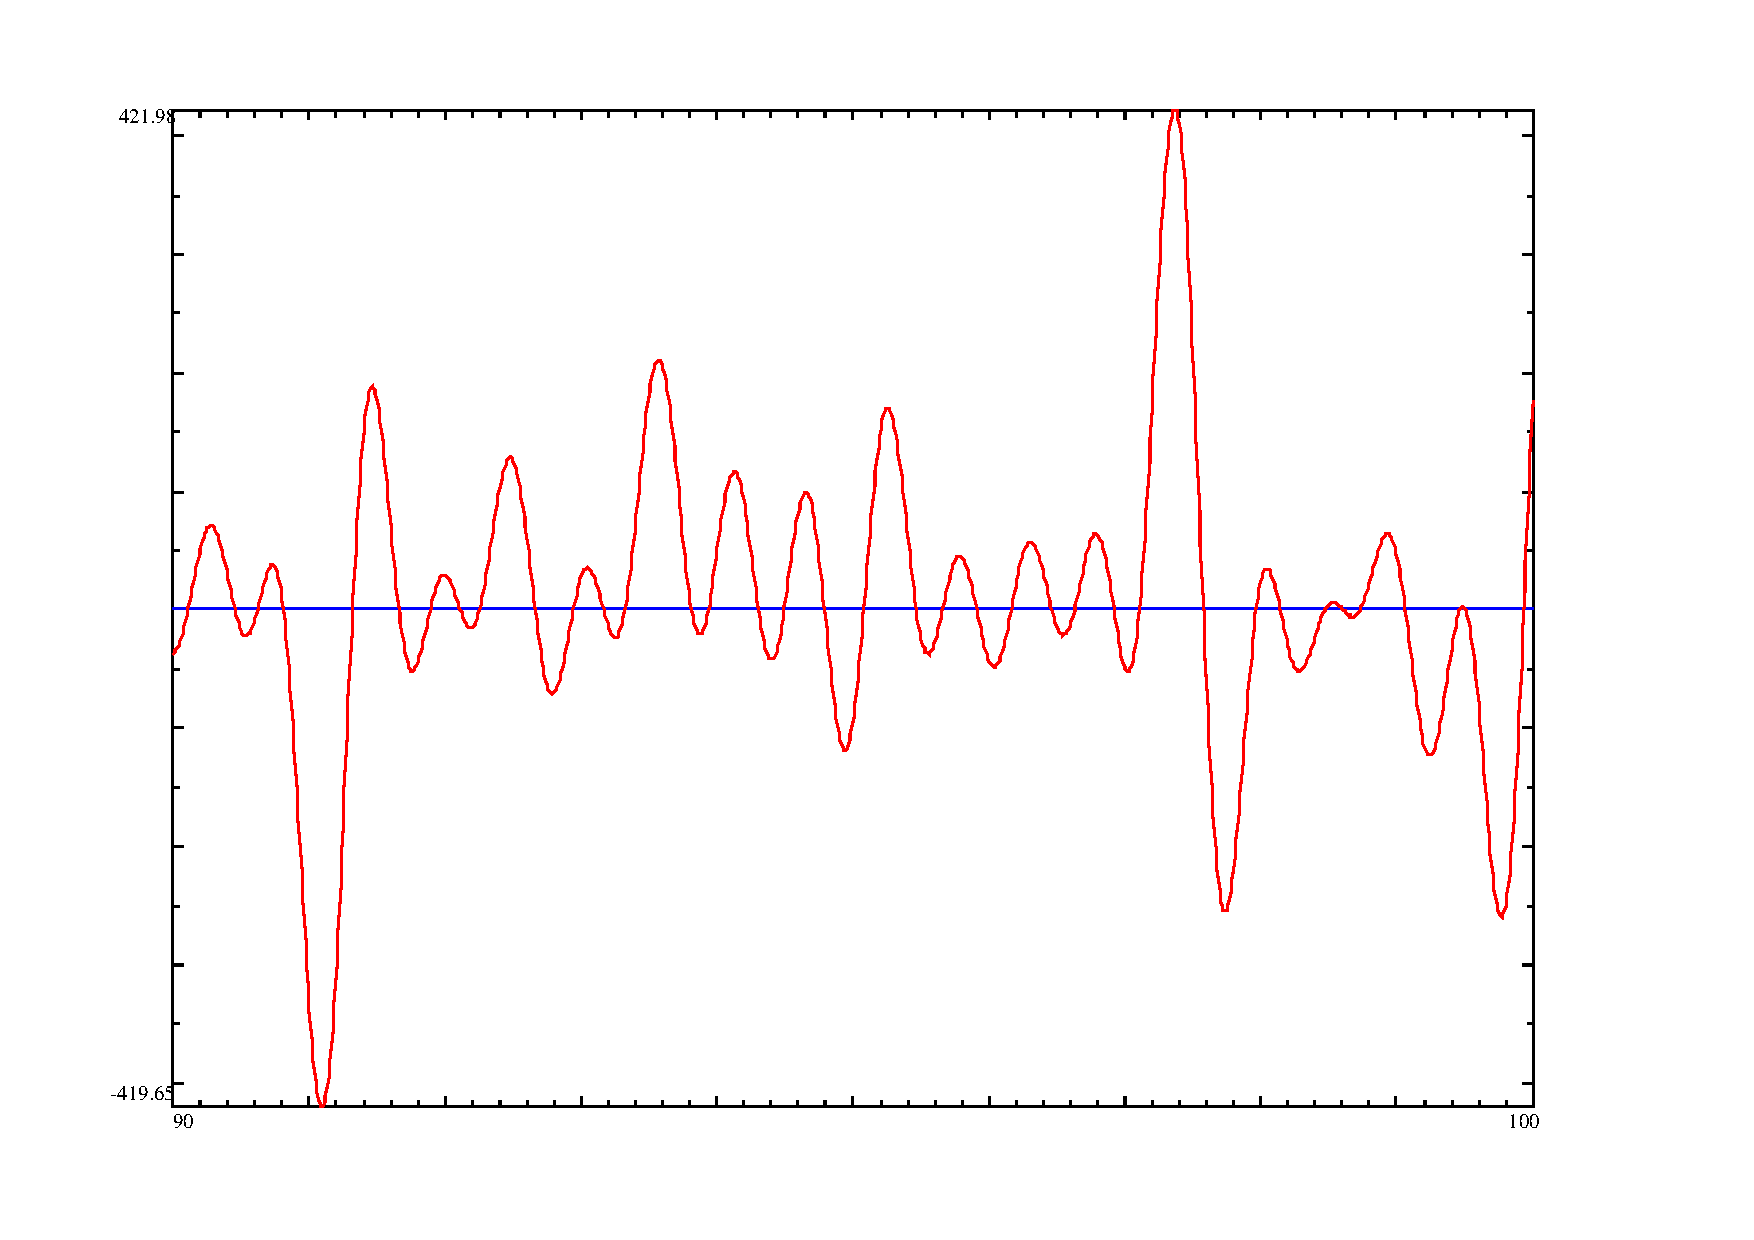
\includegraphics[scale=0.45]{L.pdf}
\end{center}
The Hardy function plotted above is a real-valued function $H(t)$ of the real
variable $t$ such that $L(1+it) = 0 \Leftrightarrow H(t) = 0$. Assuming
the Riemann hypothesis, the zeros are simple and $H$ must change sign
at each zero of $L(1+it)$, which is in fact the basis of the
\texttt{lfunzeros} algorithm. We can actually count the 37 zeros in the
graph, but two zeros at the right end of the interval are doubtful. Zooming
in shows that the graph indeed crosses the real axis twice:
\begin{verbatim}
? parploth(t = 98,100, lfunhardy(L,t))
\end{verbatim}
\begin{center}
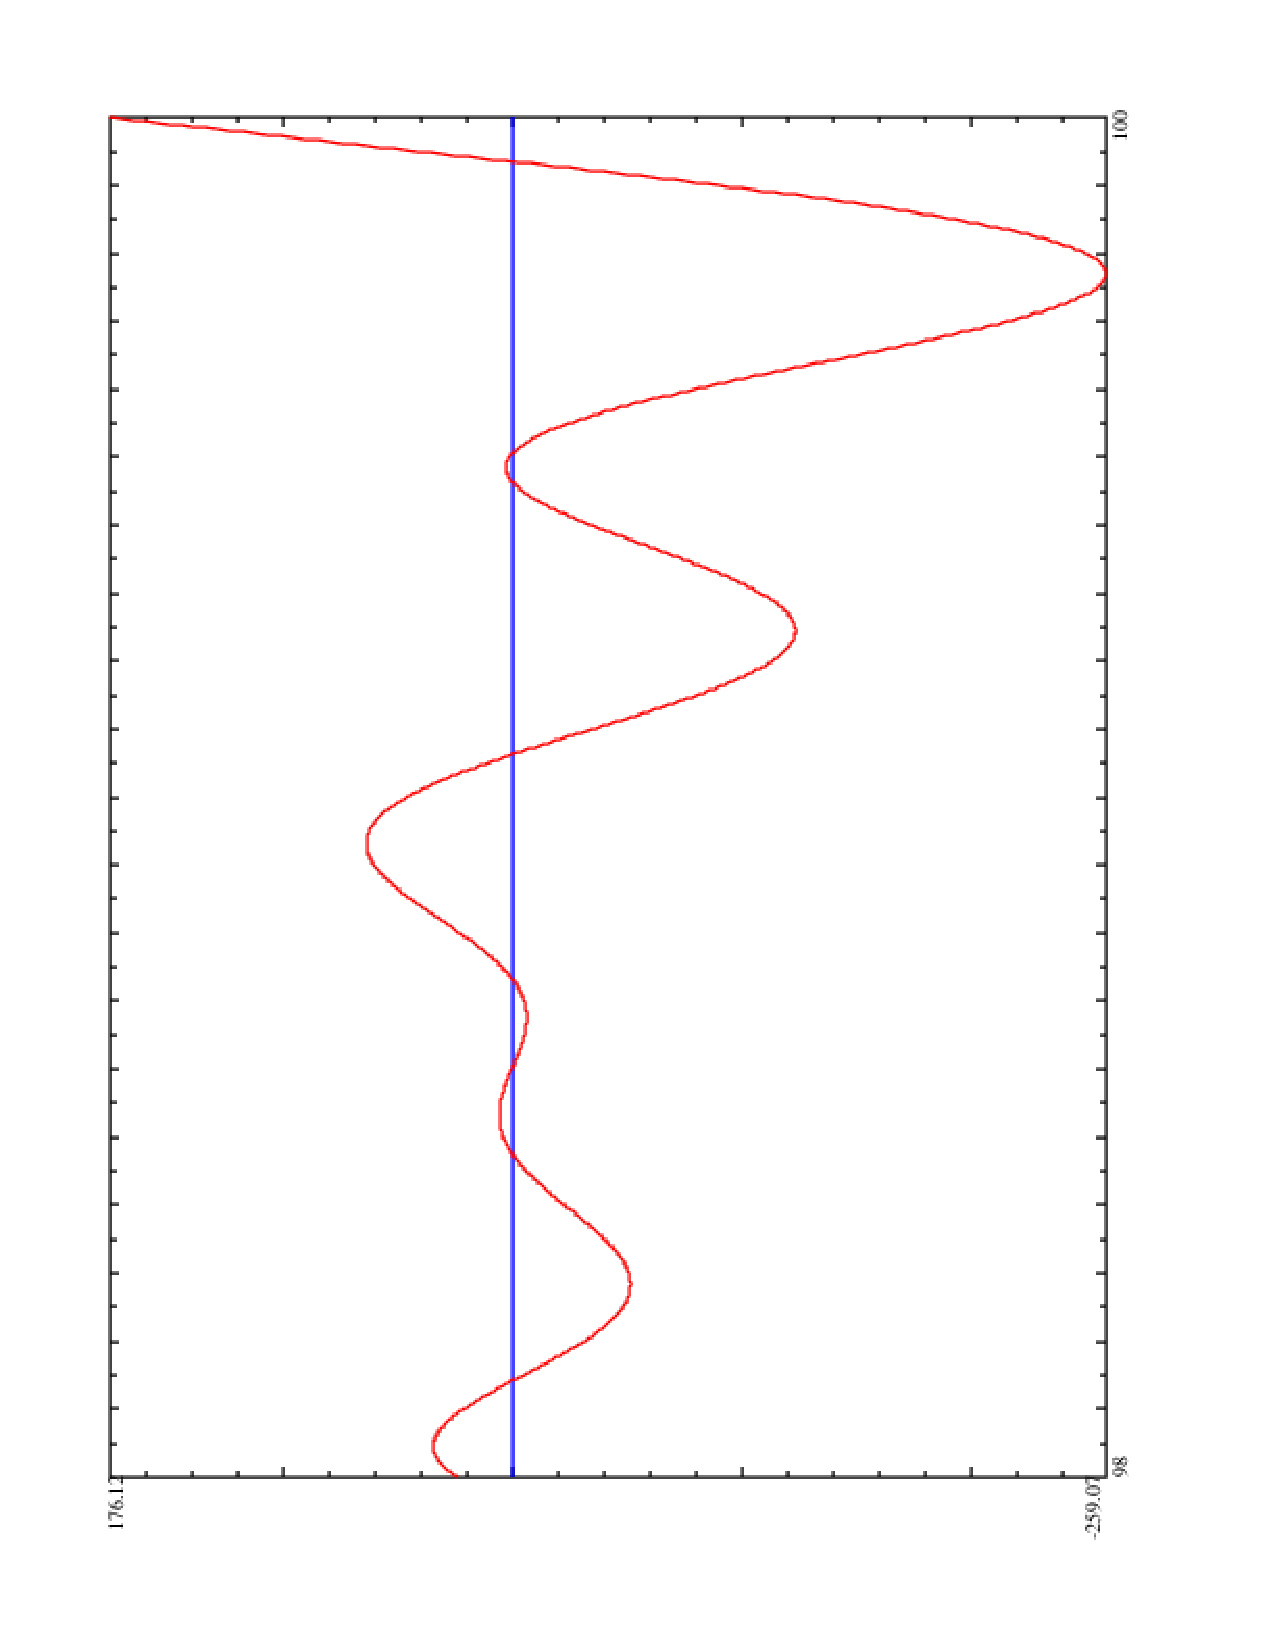
\includegraphics[scale=0.45,angle=-90]{L2.pdf}
\end{center}

The speedup profile for each individual command depends on the relative cost
of the pre- or post-processing phases. For instance testing determinants and
matrix kernels, both computed by Chinese remaindering techniques, the
perceived speedups caps around 10.8 and 5.9 respectively, instead of the
previous 13.6:

\begin{verbatim}
 n = 300; m = matrix(n,n,i,j,random(2^n)); matdet(m);
 n = 150; m = matrix(n,n+40,i,j,random(2^n)); matker(m);
\end{verbatim}
\begin{center}
\begin{tikzpicture}
\begin{axis}[
    title=Real time speedup wrt. sequential run (det/ker),
xlabel={number of threads},
ylabel={speedup},
xmin=1, xmax=32,
ymin=1, ymax=32,
]
\addplot table {ellan-threads.dat};
  \addlegendentry{ellan}
\addplot table {matdet-threads.dat};
  \addlegendentry{matdet}
\addplot table {matker-threads.dat};
  \addlegendentry{matker}
\addplot [domain=0:32]{x}
         node [pos=0.6, sloped, above left]{ideal speedup};
\end{axis}
\end{tikzpicture}
\end{center}

\noindent
The sequential times were respectively 32.3s for the determinant and
19.9s for the kernel. The difference with the previous \texttt{ellan} example
is easily explained:
\begin{enumerate}
  \item We do not know in advance the actual result size so we resort to a
    doubling strategy, which makes it harder to optimize parameters.
    In fact, since our inputs are random, the a priori bounds are actually
    sharp in this example and this strategy is a waste of time.

  \item The overhead is more inportant now since modular linear algebra
    internally involve three parallelized operations: reducing our input
    modulo many small primes $(p_i)$, the modular matrix computations and
    chinese remaindering to obtain a result modulo the product $N$ of all $p_i$.

  \item In addition, the kernel involves the rational reconstruction of basis
    vectors from modular results modulo $N$ and the check that those belong
    to the kernel, contrary to the determinant which is here known to be an
    integer and is directly guaranteed to be correct. The final check is
    currently done in the main thread; in this example, it uses 25\% of the
    real computing time, cancelling some of the parallelization gains.
    The check could be moved to the parallel section of the code but this
    causes difficulties in other examples. In any case, there is room for
    improvement here.
\end{enumerate}

\subsection{MPI}

We now write part of the commands above in a file \texttt{E.gp}:
\begin{verbatim}
E = ellinit([i,i+1], nfinit(i^2+1));
ellan(E, 10^7);
\end{verbatim}
We run the same computation non-interactively with a \texttt{gp} configured
to use MPI; note that the argument to \texttt{mpirun -np} is the number of
process slots, which is one more than the number of available secondary
threads since one slot is used by the master thread:
\begin{verbatim}
# time mpirun -np 9 gp -q < E.gp
42.97s user 0.45s system 861% cpu 5.040 total
# time mpirun -np 17 gp -q < E.gp
60.28s user 6.86s system 1527% cpu 4.394 total
# time mpirun -np 33 gp -q < E.gp
73.73s user 14.36s system 2776% cpu 3.173 total
\end{verbatim}
The overhead is more important than with POSIX
threads but we are no longer limited by the number of logical cores on a
single machine.

\subsection{External applications}

Since the MT engine is part of the \Pari library, it is available
without any additional effort to all applications and interfaces using it.
This example, taken from deliverable D4.10
(PARI/Python bindings, \texttt{cypari2}) shows how easy it is for
external applications (here IPython) to leverage the GP parallel interface:

\begin{verbatim}
In [1]: from cypari2 import Pari; pari = Pari()
In [2]: pari.default("nbthreads", 2)
In [3]: L = [2**i - 1 for i in range(1, 201)]
In [4]: %time res = pari.parapply("factor", L)
CPU times: user 6.76 s, sys: 170 ms, total: 6.93 s
Wall time: 3.6 s
\end{verbatim}

This factors a few Mersenne numbers using 2 threads, without paying attention
to sizing tasks or load balancing (some factorizations in the list are
instantaneous, some much slower). Nevertheless, we gain roughly a factor 2.

\bigskip
\bigskip

\appendix
\section{Snapshot of the documentation at the time of delivery}

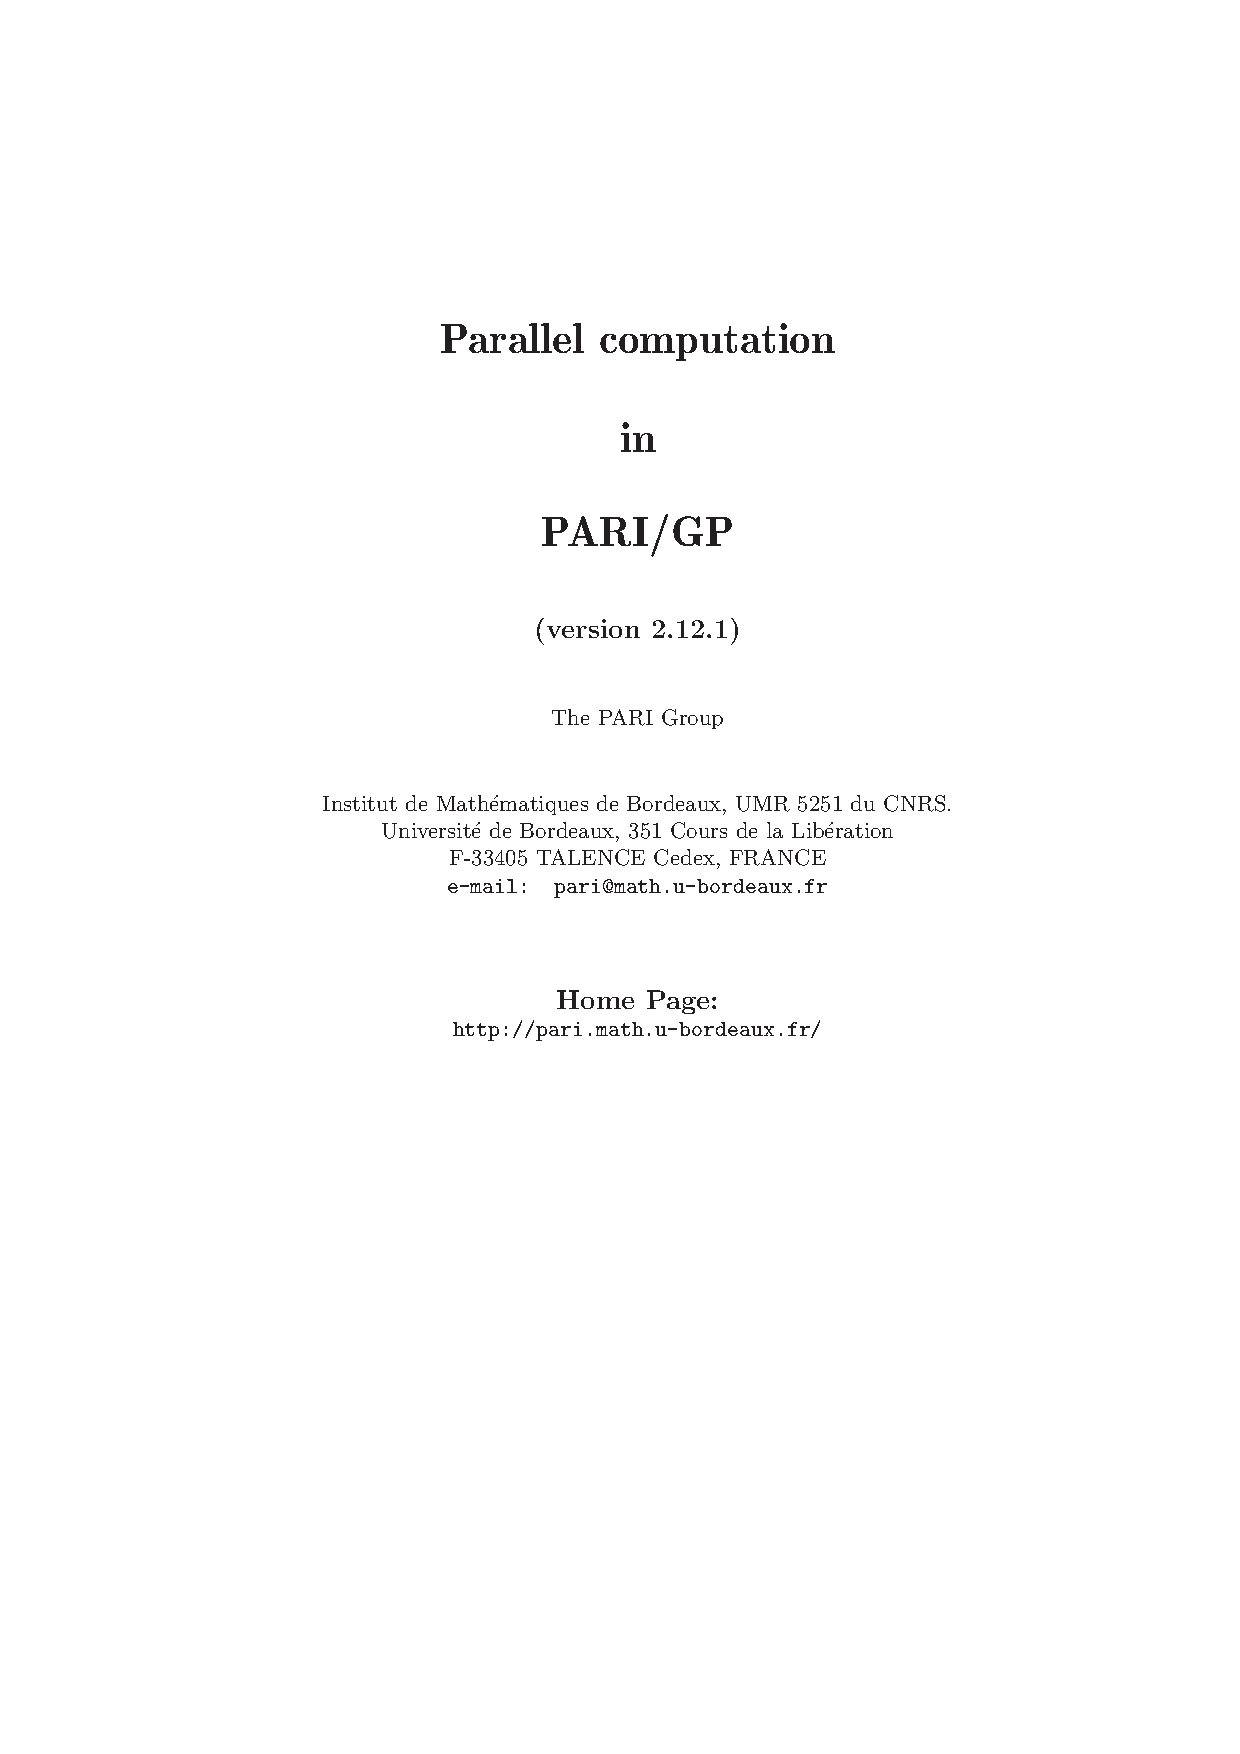
\includepdf[pages=-]{ODK-parallel.pdf}
\end{document}
